\documentclass[12pt]{article}
\usepackage[utf8]{inputenc}
\usepackage{graphicx}
\usepackage{amsmath}
\usepackage[margin=1in]{geometry}
\usepackage{indentfirst}
\usepackage{amsfonts}
%for english
\usepackage[english]{babel}
%for portuguese
%\usepackage[portuguese]{babel}
\usepackage{float}
\usepackage[usenames,dvipsnames]{color}

\usepackage{listings}
\usepackage{color}

\definecolor{mygreen}{rgb}{0,0.6,0}
\definecolor{mygray}{rgb}{0.5,0.5,0.5}
\definecolor{mymauve}{rgb}{0.58,0,0.82}

\lstset{ %
  backgroundcolor=\color{white},   % choose the background color; you must add \usepackage{color} or \usepackage{xcolor}
  basicstyle=\footnotesize,        % the size of the fonts that are used for the code
  breakatwhitespace=false,         % sets if automatic breaks should only happen at whitespace
  breaklines=true,                 % sets automatic line breaking
  captionpos=b,                    % sets the caption-position to bottom
  commentstyle=\color{mygreen},    % comment style
  deletekeywords={...},            % if you want to delete keywords from the given language
  escapeinside={\%*}{*)},          % if you want to add LaTeX within your code
  extendedchars=true,              % lets you use non-ASCII characters; for 8-bits encodings only, does not work with UTF-8
  frame=single,                    % adds a frame around the code
  keepspaces=true,                 % keeps spaces in text, useful for keeping indentation of code (possibly needs columns=flexible)
  keywordstyle=\color{blue},       % keyword style
  language=C,                 % the language of the code
  morekeywords={*,...},            % if you want to add more keywords to the set
  numbers=left,                    % where to put the line-numbers; possible values are (none, left, right)
  numbersep=5pt,                   % how far the line-numbers are from the code
  numberstyle=\tiny\color{mygray}, % the style that is used for the line-numbers
  rulecolor=\color{black},         % if not set, the frame-color may be changed on line-breaks within not-black text (e.g. comments (green here))
  showspaces=false,                % show spaces everywhere adding particular underscores; it overrides 'showstringspaces'
  showstringspaces=false,          % underline spaces within strings only
  showtabs=false,                  % show tabs within strings adding particular underscores
  stepnumber=1,                    % the step between two line-numbers. If it's 1, each line will be numbered
  stringstyle=\color{mymauve},     % string literal style
  tabsize=2,                       % sets default tabsize to 2 spaces
  title=\lstname                   % show the filename of files included with \lstinputlisting; also try caption instead of title
}




\begin{document}




\begin{titlepage}

\newcommand{\HRule}{\rule{\linewidth}{0.5mm}} 
\center 
 

\textsc{\LARGE Universidade de Coimbra}\\[1.5cm] % Name of your university/college
\textsc{\Large Departamento de Engenharia Informática}\\[4cm] % Major heading such as course name
\textsc{\large Compiladores}\\[1cm] % Minor heading such as course title


\HRule \\[0.5cm]
{ \huge \bfseries Compilador para linguagem iJava}\\[0.4cm] 
\HRule \\[8cm]
 
\begin{minipage}{0.4\textwidth}
\begin{flushleft} \large
\emph{Autor:}\\
David \textsc{Cardoso}  \\Número: 2011164039
\end{flushleft}
\end{minipage}
~
\begin{minipage}{0.4\textwidth}
\begin{flushright} \large
\emph{Autor:} \\
Bruno \textsc{Caceiro}  \\Número: 2008107991
\end{flushright}
\end{minipage}\\[2cm]

{\large \today}\\[3cm]

\vfill

\end{titlepage}



\section{Introdução}
Este projecto consiste no desenvolvimento de um compilador para a linguagem \emph{iJava} (imperative Java), que consiste num pequeno subconjunto da linguagem Java (versão 5.0). Os programas da linguagem \emph{iJava} são constituídos por uma única classe (a principal), contendo necessariamente um método \emph{main}, e podendo conter outros métodos e atributos, todos eles estáticos e (possivelmente) públicos.

O projecto foi estruturado em 3 fases, primeiramente foi feita a Análise Lexical, implementada na linguagem \emph{C} e utilizando a ferramenta \emph{lex}. A segunda fase consistiu na análise sintática, com a  construção da árvore de sintaxe abstrata e análise semântica (tabelas de símbolos, deteção de erros semânticos). No final foi feita a geração de código.

\begin{figure}[H]
       \centering
       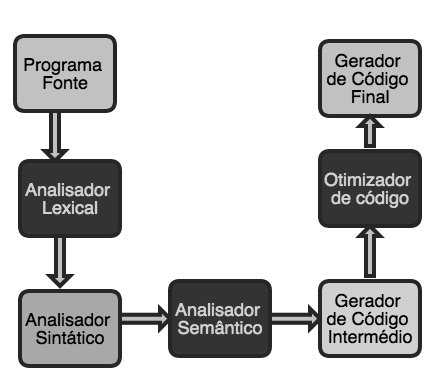
\includegraphics[keepaspectratio=true, width=300px]{fasesCompilacao.png}
       \caption{Fases de Compilação}
       \end{figure}


\section{Análise Lexical}

A Análise Lexical consiste em analisar a entrada de linhas de caracteres e produzir uma sequência de símbolos (\emph{tokens}) que podem ser manipulados mais facilmente por um \emph{parser}. É uma forma de verificar um determinado alfabeto, neste caso o alfabeto da linguagem \emph{iJava}.
Esta análise pode ser dividida em três fases:
\begin{itemize}
	\item Extração e classificação de \emph{tokens};
	\item Eliminação de delimitadores e comentários;
	\item Tratamento de erros;
\end{itemize}


\subsection{Tokens}
\begin{itemize}
	        \item \textbf{ID:} Sequências alfanuméricas começadas por uma letra, onde os símbolos "\_" e "\$" contam como letras. Maiúsculas e minúsculas são consideradas letras diferentes 
	        \item \textbf{INTLIT:} Sequências de dígitos decimais e sequências de dígitos hexadecimais (incluindo a-f e A-F) precedidas de "0x"
	        \item \textbf{BOOLLIT:} "true" \text{\textbar} "false" 
	        \item \textbf{INT:} "int"
	        \item \textbf{BOOL:} "boolean"
	        \item \textbf{NEW:} "new"
	        \item \textbf{IF:} "if"
	        \item \textbf{ELSE:} "else"
	        \item \textbf{WHILE:} "while"
	        \item \textbf{PRINT:} "System.out.println"
	        \item \textbf{PARSEINT:} "Integer.parseInt"
	        \item \textbf{CLASS:} "class"
	        \item \textbf{PUBLIC:} "public"
	        \item \textbf{STATIC:} "static"
	        \item \textbf{VOID:} "void"
	        \item \textbf{STRING:} "String"
	        \item \textbf{DOTLENGTH:} ".length"
	        \item \textbf{RETURN:} "return"
	        \item \textbf{OCURV:} "("
	        \item \textbf{CCURV:} ")"
	        \item \textbf{OBRACE} "\{"
	        \item \textbf{CBRACE:} "\}"
	        \item \textbf{OSQUARE:} "["
	        \item \textbf{CSQUARE:} "]"	 
	      \end{itemize}
	      \pagebreak
	    Foi necessário separar alguns \emph{tokens} devido às diferentes prioridades que cada operador tem.
		\begin{itemize}  
	        \item \textbf{OP1:} "\&\&"  
	        \item \textbf{OP1OR:} "\text{\textbar} \text{\textbar}"
	        \item \textbf{OP2:} "\textless" \text{\textbar} "\textgreater" \text{\textbar} "\textless=" \text{\textbar} "\textgreater="
	        \item \textbf{OP2EQS:} "==" \text{\textbar} "!="	        
	        \item \textbf{OP3:} "+" \text{\textbar} "-"
	        \item \textbf{OP4:} "*" \text{\textbar} "/" \text{\textbar} "\%"
	        \item \textbf{NOT:} "!"
	        \item \textbf{ASSIGN:} "="
	        \item \textbf{SEMIC:} ";"
	        \item \textbf{COMMA:} ","
	        \item \textbf{RESERVED:} O \emph{iJava} é um subconjunto da linguagem \emph{Java}, como tal, existe um conjunto de funcionalidades que embora não sejam suportadas, têm de ser consideradas. Assim, foi necessário tratar todo um conjunto de palavras reservadas de forma a permitir que sejam lexicalmente válidas mas não sintaticamente. 
	       	            \begin{itemize}
	       	                \item abstract
	       	                \text{\textbar} assert 
	       	                \text{\textbar} break 
	       	                \text{\textbar} byte 
	       	                \text{\textbar} case 
	       	                \text{\textbar} catch 
	       	                \text{\textbar} char 
	       	                \text{\textbar} const 
	       	                \text{\textbar} continue
	       	                 \text{\textbar} default 
	       	                 \text{\textbar} do 
	       	                 \text{\textbar} double
	       	                 \text{\textbar} enum 
	       	                 \text{\textbar} extends 
	       	                 \text{\textbar} final 
	       	                 \text{\textbar} finally 
	       	                 \text{\textbar} float 
	       	                 \text{\textbar} for 
	       	                 \text{\textbar} goto 
	       	                 \text{\textbar} implements 
	       	                 \text{\textbar} import 
	       	                 \text{\textbar} instanceof
	       	                 \text{\textbar} interface 
	       	                 \text{\textbar} long
	       	                 \text{\textbar} native
	       	                 \text{\textbar} package
	       	                 \text{\textbar} private 
	       	                 \text{\textbar} protected 
	       	                 \text{\textbar} short 
	       	                 \text{\textbar} strictfp
	       	                 \text{\textbar} super 
	       	                 \text{\textbar} switch 
	       	                 \text{\textbar} synchronized 
	       	                 \text{\textbar} this 
	       	                 \text{\textbar} throw 
	       	                 \text{\textbar} throws 
	       	                 \text{\textbar} transient 
	       	                 \text{\textbar} try
	       	                 \text{\textbar} volatile
		       	             \text{\textbar} null
	       	                 \text{\textbar} ++
	       	                 \text{\textbar} --
	       	            \end{itemize}      	        
		\end{itemize}
		
		
		\subsubsection{Tratamento de Erros}
		Se forem detectados erros lexicais no ficheiro de entrada então é impressa uma mensagem de erro no \emph{stdout}:
		\begin{itemize}
            \item "Line\textless num linha\textgreater,col\textless num coluna\textgreater:illegal character('\textless c \textgreater'\textbackslash n)"
            \item "Line\textless num linha\textgreater,col\textless num coluna\textgreater:unterminated comment\textbackslash n"
        \end{itemize}
		






\section{Análise Sintática e Semântica}

\subsection{Gramática}

A gramática é a maneira formal de especificar a sintaxe de uma linguagem. 
Desenvolver uma gramática não ambígua é um dos passos mais importantes para o sucesso do compilador. Para a gramática da linguagem \emph{iJava} usámos a notação \textbf{EBNF} \emph{(Extended Backus Naur Form)}. 
A gramática que nos foi dada era ambígua e por isso tivémos de efectuar diversas alterações para permiter a análise sintática ascendente com o \emph{yacc}.\\


\begin{itemize}
  \item[] START $\longrightarrow$ $CLASS$ $ID$  $OBRACE$ field\_or\_method\_declaration $CBRACE$
\\
  \item[]  field\_or\_method\_declaration $\longrightarrow$  $FieldDecl$ field\_or\_method\_declaration \par$|$ $MethodDecl$  field\_or\_method\_declaration
\\   
  \item[] $FieldDecl$ $\longrightarrow$ $STATIC$ $VarDecl$  VarDecl\_REPETITION
  \\
  \item[] $MethodDecl$ $\longrightarrow$ $PUBLIC$ $STATIC$ method\_type\_declaration $ID$  $OCURV$ FormalParams $CCURV$ $OBRACE$ VarDecl\_REPETITION statement\_declaration\_REPETITION $CBRACE$
  \\
  \item[] method\_type\_declaration $\longrightarrow$ Type 
  \begin{itemize}
	\item[] $|$ $VOID$
  \end{itemize}

  \item[] FormalParams $\longrightarrow$ Type $ID$ several\_FormalParams 
  \begin{itemize}
 	\item[]$|$ $STRING$    $OSQUARE$ $CSQUARE$  $ID$  
  \end{itemize}
  
  \item[] several\_FormalParams $\longrightarrow$ $COMMA$ Type $ID$ several\_FormalParams  
  \\
  \item[] VarDecl\_REPETITION $\longrightarrow$ VarDecl VarDecl\_REPETITION 
 \\
  \item[] VarDecl $\longrightarrow$ Type $ID$ several\_var\_decl\_in\_same\_instructionOPTIONAL $SEMIC$
  \\
  \item[]several\_var\_decl\_in\_same\_instructionOPTIONAL $\longrightarrow$ $COMMA$ $ID$ several\_var\_decl\_in\_same\_instructionOPTIONAL 
  \\
  \item[]Type $\longrightarrow$ $INT$ $OSQUARE$ $CSQUARE$ 
  \begin{itemize}
  \item[]$|$ $BOOL$ $OSQUARE$ $CSQUARE$ 
  \\$|$ $INT$ 
  \\$|$ $BOOL$
  \end{itemize}
  
  \item[] statement\_declaration\_REPETITION $\longrightarrow$ Statement statement\_declaration\_REPETITION
  \\
  \item[] Statement $\longrightarrow$ $OBRACE$ several\_statement $CBRACE$
  \begin{itemize}
  \item[]$|$ $IF$ $OCURV$ Expr $CCURV$ Statement $\%prec$ $IFX$ 
  \\$|$ $IF$ $OCURV$ Expr $CCURV$ Statement $ELSE$ Statement 
  \\$|$ $WHILE$ $OCURV$ Expr $CCURV$ Statement 
  \\$|$ $PRINT$ $OCURV$ Expr $CCURV$ $SEMIC$ 
  \\$|$ $ID$ array\_indexOPTIONAL $ASSIGN$ Expr $SEMIC$ 
  \\$|$ $RETURN$ return\_expression $SEMIC$  
    \end{itemize}
  
  \item[] several\_statement $\longrightarrow$ Statement several\_statement  
  \\
  \item[] array\_indexOPTIONAL $\longrightarrow$  $OSQUARE$ Expr $CSQUARE$
  \\
  \item[] return\_expression $\longrightarrow$  Expr
  \\
  \item[] IndexableExpr $\longrightarrow$ $ID$ 
  \begin{itemize}
  \item[]$|$ $INTLIT$ $BOOLLIT$ $ID$ $OCURV$ Args\_OPTIONAL $CCURV$ 
  \\$|$ $OCURV$ Expr $CCURV$ 
  \\$|$ Expr $DOTLENGTH$ 
  \\$|$ IndexableExpr $OSQUARE$ Expr $CSQUARE$ 
  \\$|$ $PARSEINT$ $OCURV$ $ID$ $OSQUARE$ Expr $CSQUARE$ $CCURV$
    \end{itemize}

  \item[] Expr $\longrightarrow$ Expr $OP1$ Expr $\%prec$ $OP1$ 
  \begin{itemize}
		\item[] $|$      Expr $OP1OR$ Expr $\%prec$ $OP1OR$
		\\$|$ Expr $OP4$ Expr $\%prec$ $OP4$ 
		\\$|$ Expr $OP3$ Expr $\%prec$ $OP3$  
		\\$|$ Expr $OP2$ Expr $\%prec$ $OP2$ 
		\\$|$ Expr $OP2EQS$ Expr $\%prec$ $OP2EQS$
		\\$|$ $OP3$ Expr $\%prec$ $NOT$
		\\$|$ $NOT$ Expr $\%prec$ $NOT$
		\\$|$ $NEW$ $INT$ $OSQUARE$ Expr $CSQUARE$
		\\$|$ $NEW$ $BOOL$ $OSQUARE$ Expr $CSQUARE$
		\\$|$ IndexableExpr
  \end{itemize}

  \item[] Args\_OPTIONAL $\longrightarrow$ Args
  \\
  \item[] Args $\longrightarrow$ Expr comma\_expr
  \\
  \item[] comma\_expr $\longrightarrow$ $COMMA$ Expr comma\_expr               
  
  
\end{itemize}


\subsection{Árvore de Sintaxe Abstrata}

Estruturas utilizadas para a criação da árvore de sintaxe abstrata
\begin{lstlisting}
/* General Node */
typedef struct _Node
{
    //Type of the Node (to identify the type of the node)
	NodeType n_type;

    //Type of the Struct (Int, Void, String,...)
	Type type;

    //Id or list of id's
    listID* id;

    //The tree next nodes (the case of if)
    struct _Node* n1;
    struct _Node* n2;
    struct _Node* n3;

    //Next node
    struct _Node* next;

    //Literals (to store the values)
    char* value;

    char isStatic;
}Node;


//Linked list of ID's (for multiple declaration of variables)
typedef struct _idList
{
	char* id;
	struct _idList* next;
}listID;

\end{lstlisting}
 


\subsection{Tratamento de Erros Lexicais}

\subsection{Análise Semântica}

\subsection{Tabela de Símbolos}

\subsection{Tratamento de Erros Semânticos}









	
	


\end{document}